\section{Introduction}
\begin{frame}{Engineering Endeavours}
\begin{minipage}{0.45\textwidth}
  \begin{itemize}
    \item Limited world 
    \item Performance 
    \item Reliability 
  \end{itemize}
\end{minipage}%
\hspace{1cm}
\begin{minipage}{0.45\textwidth}
    \centering
    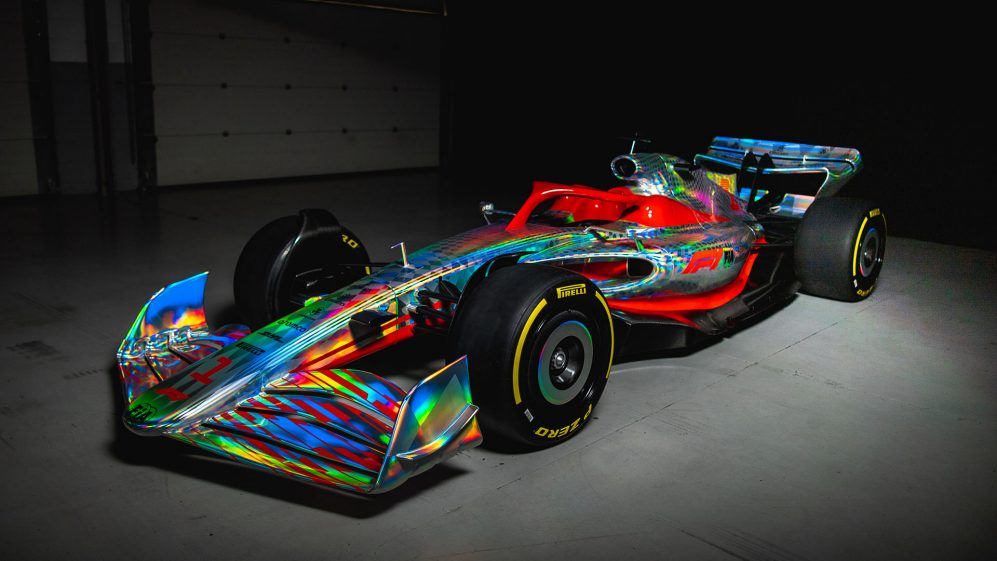
\includegraphics[width=0.8\textwidth]{Figures/intro/f1.jpg}
\end{minipage}
\end{frame}


\begin{frame}{Material Behaviour}
\begin{minipage}{0.45\textwidth}
  \begin{itemize}
    \item<1> Baby's understanding 
    \item<2> What do grown ups do? 
  \end{itemize}
\end{minipage}%
\hspace{1cm}
\begin{minipage}{0.45\textwidth}
    \centering
    \includegraphics<1>[width=0.6\textwidth]{Figures/intro/baby.jpeg}
    \only<2>{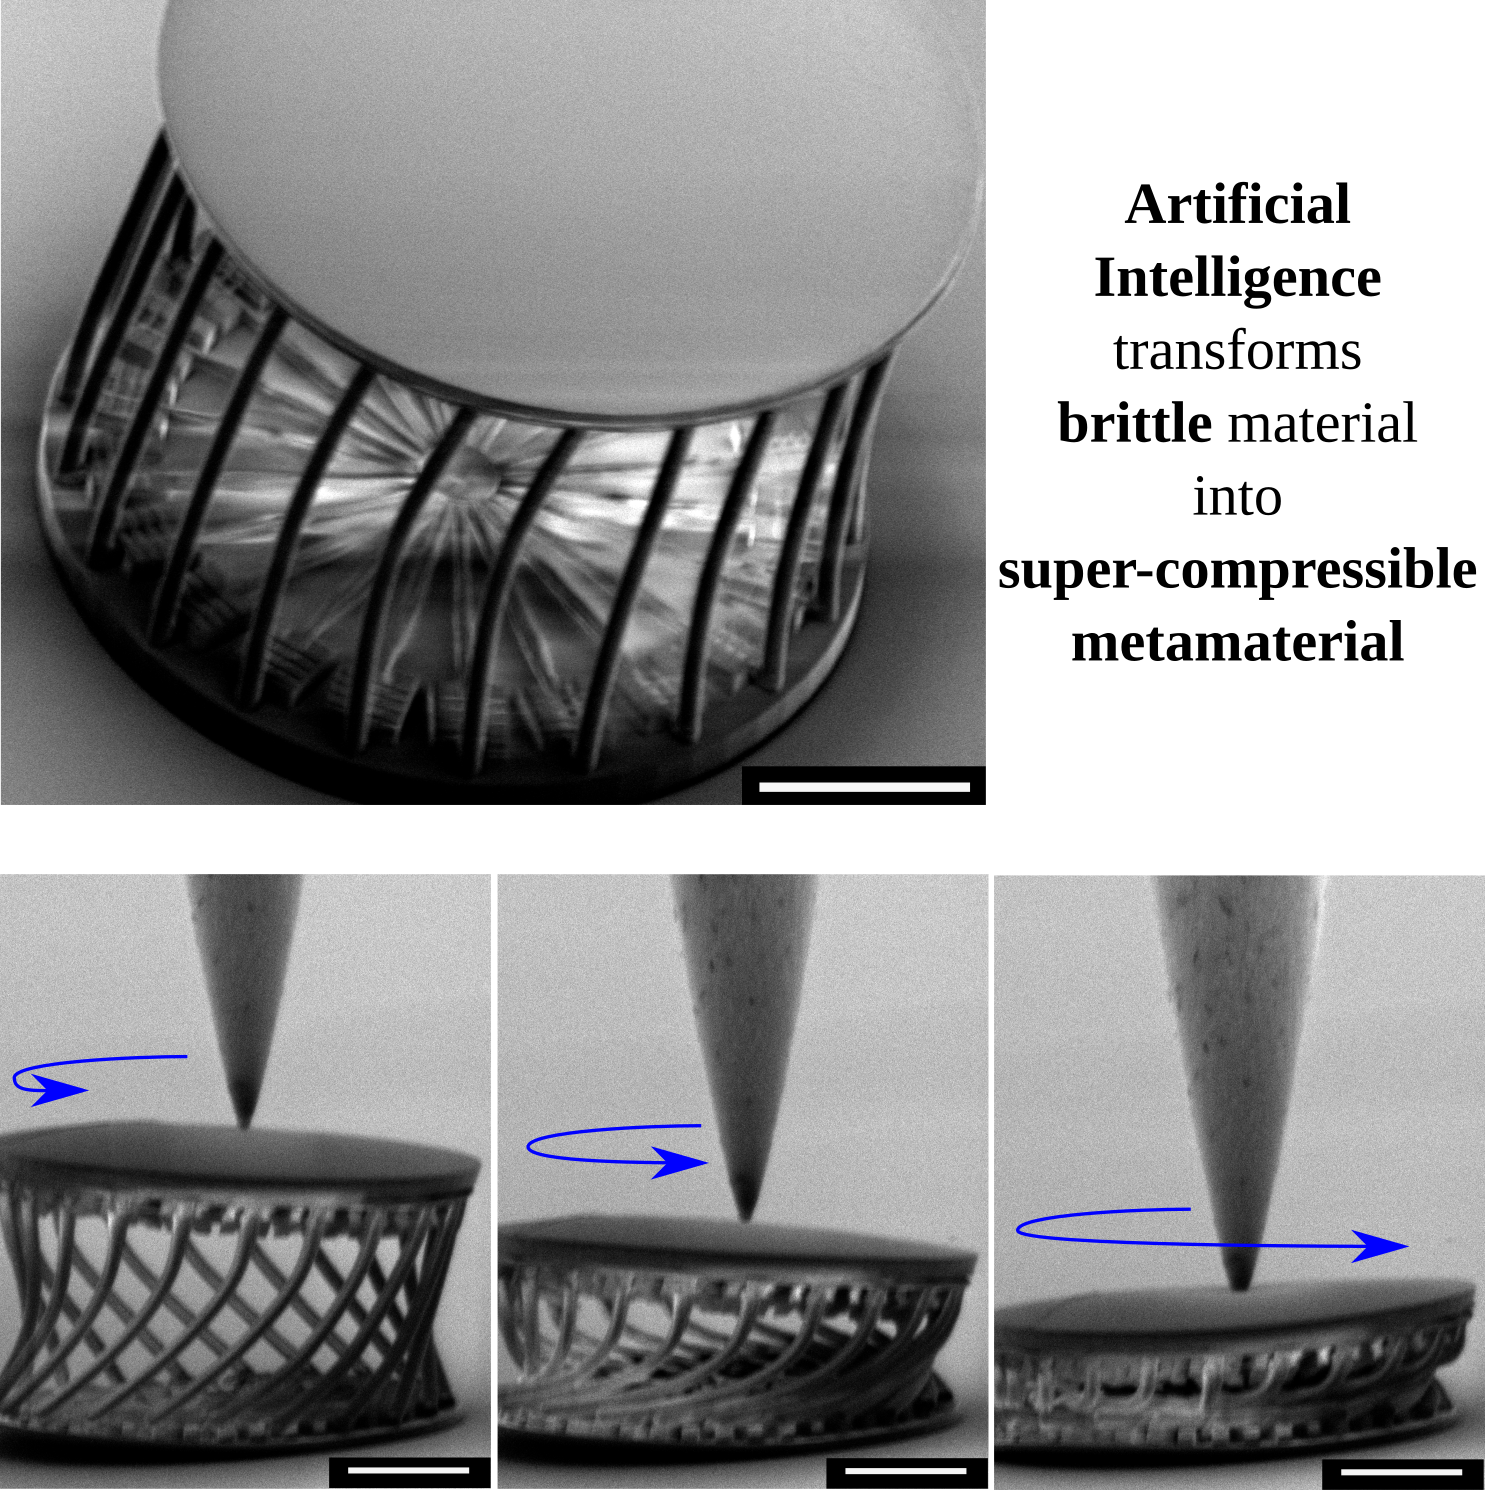
\includegraphics[width=0.8\textwidth]{Figures/intro/lab.png}\cite{Bessa2019a}}
\end{minipage}
\end{frame}

\section{Modeling Composites}
\begin{frame}{Composites}
\begin{minipage}{0.45\textwidth}
  \begin{block}{\color{White}Experimental}<2>
    \begin{itemize}
      \item <2> Time and money limitations
    \end{itemize}
  \end{block} 
  \begin{block}{\color{White}Numerical Analysis}<2-4>
    \begin{itemize}
      \item <3> Multi-scale venture
      \item <4> The Finite Element Method
    \end{itemize}
  \end{block} 
\end{minipage}%
\hspace{1cm}
\begin{minipage}{0.45\textwidth}
    \centering
    \includegraphics<1-3>[width=0.8\textwidth]{Figures/intro/scales.pdf}
    \includegraphics<4>[width=0.8\textwidth]{Figures/intro/link.png}
\end{minipage}
\end{frame}

\begin{frame}{Numerical Modeling Composites}
\begin{minipage}{0.45\textwidth}
  \begin{block}{\color{White}FE$^2$ (Concurrent FEM)\cite{Feyel2003}}<1-4>
    \begin{itemize}
      \item <1> Couple scales \cite{Miehe2002, Miehe1999}
      \item <2> Average the response
      \item <3> Is it enough?
    \end{itemize}
  \end{block} 
\end{minipage}%
\hspace{1cm}
\begin{minipage}{0.45\textwidth}
    \centering
    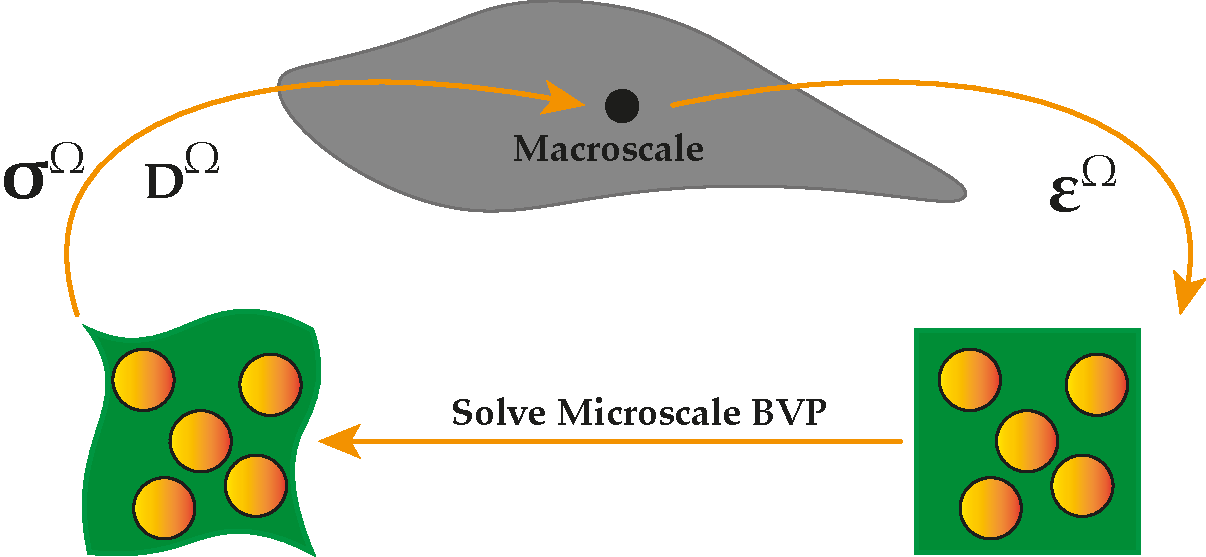
\includegraphics[width=0.8\textwidth]{Figures/intro/FE2.pdf}
\end{minipage}
\end{frame}

\begin{frame}{Numerical Modeling Composites}
\begin{minipage}{0.45\textwidth}
  \begin{block}{\color{White}Surrogate Modeling}<1-2>
    \begin{itemize}
      \item <1> Tackle computational burden
      \item <2> Keep fidelity of FE$^2$
    \end{itemize}
  \end{block} 
\end{minipage}%
\hspace{1cm}
\begin{minipage}{0.45\textwidth}
    \centering
    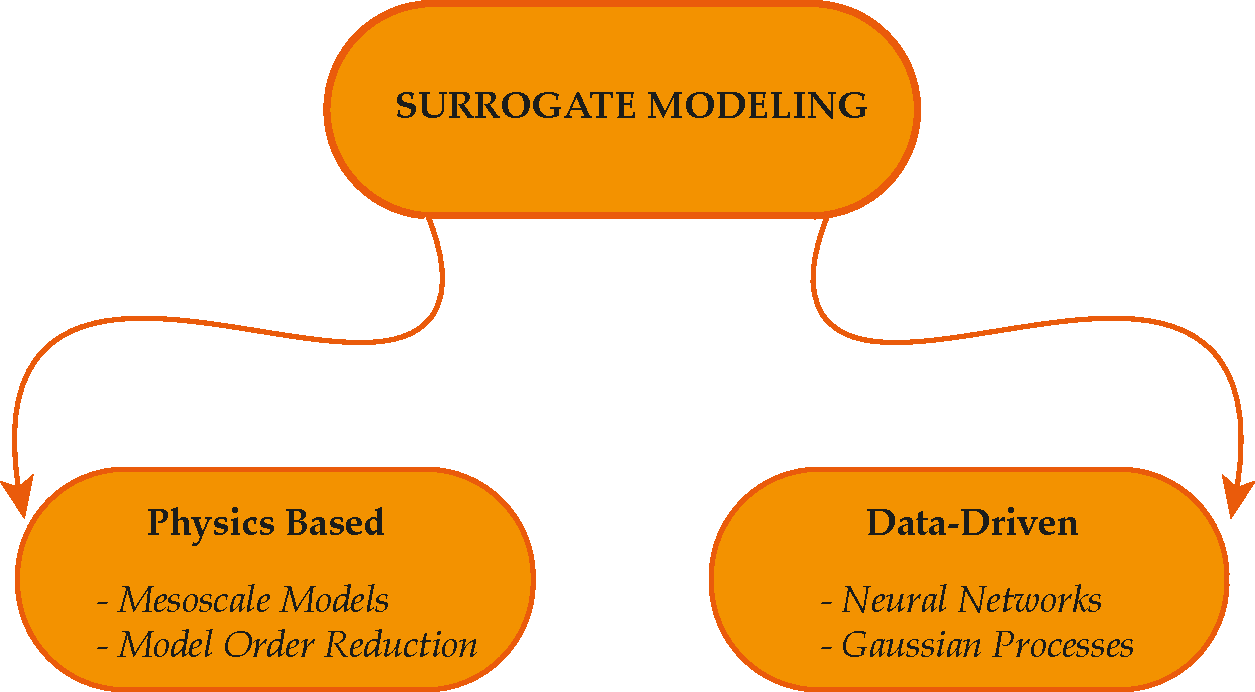
\includegraphics[width=0.8\textwidth]{Figures/intro/surrogate.pdf}
\end{minipage}
\end{frame}



